\appendix
\setcounter{table}{0}\renewcommand{\thetable}{S\arabic{table}}
\setcounter{figure}{0}\renewcommand{\thefigure}{S\arabic{figure}}
\setcounter{equation}{0}\renewcommand{\theequation}{S\arabic{equation}}
\setcounter{algorithm}{0}\renewcommand{\thealgorithm}{S\arabic{algorithm}}
\providecommand{\MipNeRF}{\emph{Mip-NeRF~360}\xspace}
\providecommand{\TandT}{\emph{Tanks and Temples}\xspace}
\providecommand{\DeepBlending}{\emph{Deep Blending}\xspace}
\providecommand{\NeRFSyn}{\emph{NeRF-Synthetic}\xspace}

Sec.~\ref{sup:impl} gives the algorithm and the implementation details. Sec.~\ref{sup:results} gives the results for all datasets, scenes and targets. Sec.~\ref{sup:codec} analyzes the codec. Sec.~\ref{sup:training} analyzes the rate-controlled training and the time of the full pipeline. Sec.~\ref{sup:qual} compares full test views with error maps. The code of the full pipeline is in the supplementary archive.

%=====================================================================
\section{Algorithm and implementation details}
\label{sup:impl}

Algorithm~\ref{sup:alg} summarizes \BM. The equations are those of Sec.~3.3 of the paper.

\begin{algorithm}[h]
\caption{\BM for a target file size $T$}
\label{sup:alg}
\small
\begin{algorithmic}[1]
\Require images, target $T$, default $b_v$, $b_f$, $R_0$
\For{iteration $i = 1 \dots 30\text{k}$}
  \State one training step of \MS; accumulate $e_t$
  \If{$i \le 10\text{k}$ and $i$ is a densification step}
    \State probe (every 1k, once pruning has started) $\rightarrow b_v, R_0$
    \State $V^\star \gets$ Eq.~(3); \ $n \gets$ Eq.~(4)
    \State split the $n$ triangles with the largest $e_t$
  \EndIf
  \If{$i = 11\text{k}$} restricted Delaunay triangulation \EndIf
  \If{$12.5\text{k} \le i \le 29.5\text{k}$ and $i$ is a multiple of 500}
    \State probe $\rightarrow R, b_v, b_f$; \ $E \gets R - T$
    \If{$E > 0$}
      \State collapse edges by increasing $c_{uv}$ (Eq.~(5)) until $\sum \Delta R_{uv} \ge E$
    \EndIf
  \EndIf
\EndFor
\State fine-tune the colors for 3{,}000 iterations
\State build the codebooks ($k$-means, refinement); encode $\rightarrow$ one file
\end{algorithmic}
\end{algorithm}

\noindent\textbf{Fine-tuning before coding.} Every mesh that we code is first fine-tuned for 3{,}000 iterations with the positions and the connectivity frozen; only the DC colors and the SH coefficients are updated. This applies to \BM, to \MSc and to the meshes from collapse after training. The 30k training iterations do not include these 3{,}000 iterations. The FP32 model is evaluated as \MS writes it.

\noindent\textbf{Phase~1.} Four details complete Sec.~3.3 of the paper. (i) \MS limits the growth of each densification step, and it excludes triangles that are too small in area or in the image. Both rules stay active, so the number of split triangles is the smaller of $n$ in Eq.~(4) of the paper and the limit of \MS. (ii) \MS also splits the largest triangles at every step; this is unchanged. (iii) The $n$ triangles are selected through a threshold on $e_t$ that is computed from the errors of the previous step, so the number of triangles that are split can differ slightly from $n$. (iv) $\sigma$ is the mean of the last three measurements, and it is 0.5 before the first one.

\noindent\textbf{Phase~2.} One round collapses at most 15\% of the vertices. When the excess $E$ needs more, the rest is removed in the next round. This happened in the first round of 2 of the 65 runs on the captured scenes.

\noindent\textbf{Final codebooks.} After $k$-means on 65{,}536 sampled vertices (8 iterations), the codebooks are updated by 4 more iterations over all vertices (2 in the size probe). The 400 refinement steps update the codewords of both codebooks and the DC colors. The positions and the indices $i_v$, $j_v$ are fixed.

\noindent\textbf{Position precision.} Table~\ref{sup:tab:bits} lists the number of bits per axis for every scene. With these values, the grid step along the longest axis is between 0.4\% and 9\% of the median edge length (measured on the meshes of Table~4 of the paper).

\begin{table}[!htb]\centering\footnotesize
\caption{\textbf{Position bits per axis.}}
\label{sup:tab:bits}
\begin{tabular}{@{}lc@{}}
\toprule
scenes & bits \\
\midrule
room; the 8 objects of \NeRFSyn & 14 \\
counter, bonsai, garden, flowers; drjohnson, playroom & 15 \\
kitchen, bicycle, stump, treehill & 16 \\
truck, train & 18 \\
\bottomrule
\end{tabular}
\end{table}

\begin{table*}[!t]\centering\footnotesize
\caption{\textbf{\BM on every captured scene}: file size (MB) / PSNR (dB) at the five targets, one run each, and the FP32 model of \MS.}
\label{sup:tab:perscene}
\begin{tabular}{@{}lcccccc@{}}
\toprule
scene & FP32 & 5 MB & 7.5 MB & 10 MB & 15 MB & 20 MB \\
\midrule
bicycle & 680 / 23.03 & 4.74 / 21.93 & 7.26 / 22.25 & 9.78 / 22.51 & 14.82 / 22.75 & 19.86 / 22.89 \\
flowers & 668 / 19.45 & 4.86 / 18.78 & 7.31 / 18.99 & 9.83 / 19.11 & 14.89 / 19.17 & 19.95 / 19.19 \\
garden & 740 / 24.73 & 4.91 / 22.75 & 7.43 / 23.32 & 10.00 / 23.67 & 15.02 / 24.10 & 19.99 / 24.34 \\
stump & 698 / 24.93 & 4.70 / 23.34 & 7.18 / 23.76 & 9.64 / 24.01 & 14.73 / 24.28 & 19.71 / 24.48 \\
treehill & 692 / 20.39 & 4.73 / 20.14 & 7.26 / 20.43 & 9.73 / 20.33 & 14.78 / 20.58 & 19.81 / 20.39 \\
room & 597 / 28.48 & 4.91 / 27.34 & 7.30 / 27.59 & 9.99 / 27.99 & 15.02 / 28.26 & 19.56 / 28.18 \\
counter & 520 / 26.48 & 4.97 / 25.19 & 7.51 / 25.59 & 10.06 / 25.71 & 15.02 / 25.91 & 20.02 / 26.03 \\
kitchen & 507 / 27.46 & 5.00 / 25.32 & 7.51 / 26.10 & 10.01 / 26.41 & 15.06 / 26.85 & 20.05 / 27.06 \\
bonsai & 678 / 28.28 & 4.87 / 26.01 & 7.42 / 26.43 & 9.79 / 26.80 & 14.97 / 27.49 & 20.27 / 27.61 \\
\midrule
truck & 432 / 22.39 & 4.94 / 21.71 & 7.44 / 22.05 & 9.90 / 22.25 & 15.00 / 22.44 & 19.96 / 22.44 \\
train & 485 / 18.90 & 4.98 / 18.46 & 7.46 / 18.67 & 9.98 / 18.77 & 15.03 / 18.90 & 20.06 / 18.84 \\
\midrule
drjohnson & 778 / 26.74 & 4.98 / 25.48 & 7.47 / 25.96 & 9.92 / 26.14 & 14.87 / 26.29 & 19.76 / 26.51 \\
playroom & 765 / 27.72 & 4.99 / 26.60 & 7.14 / 26.83 & 9.94 / 27.25 & 14.77 / 27.38 & 20.11 / 27.50 \\
\bottomrule
\end{tabular}
\end{table*}

\noindent\textbf{\NeRFSyn.} \MS is trained with a black background on this dataset. Its quality on the test views is highest some time after the triangulation and then decreases. For every model that we train on this dataset (\BM, \MSc and the FP32 model), we therefore save the model every 1{,}000 iterations from 12k on, and keep the one with the highest PSNR on the validation views of the dataset. The test views are not used for this choice. The other three datasets use the model at 30k.

\noindent\textbf{Bjontegaard deltas.} A curve is the set of points of one method on one scene, with a piecewise-linear interpolation over the logarithm of the file size. For a baseline codec, which has three SH precisions per mesh, we keep the points that no smaller file exceeds in PSNR. BD-PSNR is the mean difference over the range of file sizes that the two curves share, and BD-rate over the range of PSNR that they share. In Table~1 (bottom) of the paper, the BD-rate is averaged over the 20 scenes where the two curves share a PSNR range (7 of the 8 objects; on ficus they do not overlap). The BD-PSNR is averaged over all 21 scenes.

\noindent\textbf{Rendering time.} The times in Sec.~4.4 are measured in Chrome on a laptop (Apple M2 Max) with a canvas of $1920\times958$ pixels. Each of 300 frames is forced to complete by reading back one pixel, so the times are not limited by the display rate. Our viewer evaluates the SH of degree 3 in the vertex shader. For 3DGS we use a public WebGL viewer~\cite{splatviewer} with the models that it provides for garden and bicycle (5.8 and 6.1 million Gaussians). This viewer renders the base color only and sorts the Gaussians in a separate thread; one sort takes 35 to 47~ms and is not included in the frame time.

%=====================================================================
\section{Additional results}
\label{sup:results}

\subsection{All targets and all scenes}
\begin{figure*}[!tp]\centering
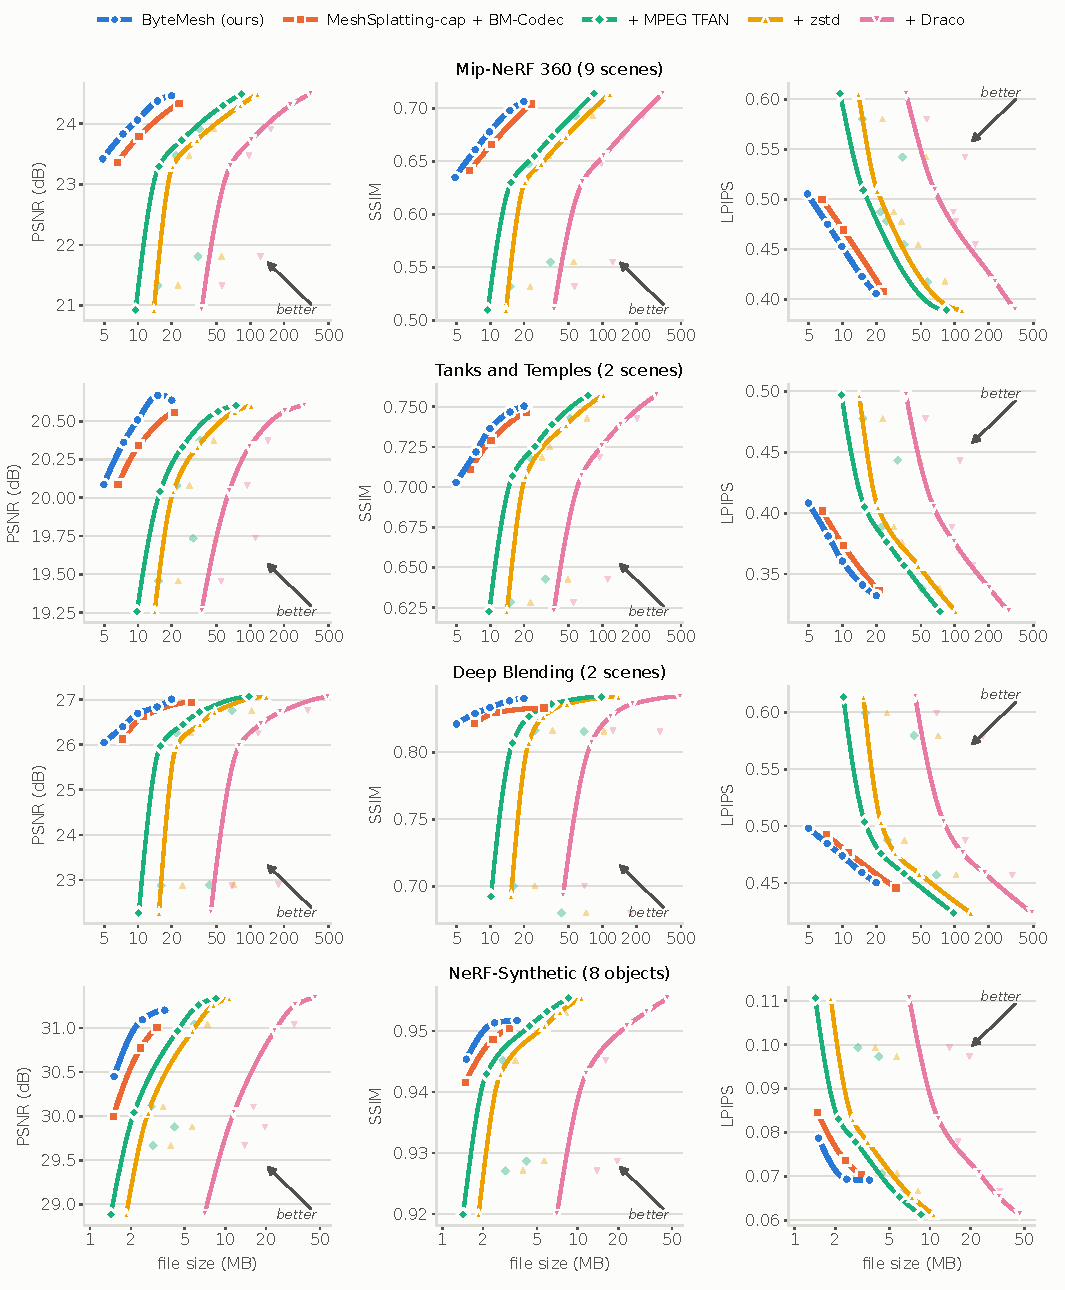
\includegraphics[width=\linewidth]{figures/fig_rd_all_v2.pdf}
\caption{\textbf{Rate--distortion on the four datasets in PSNR, SSIM and LPIPS} (mean over the scenes of each dataset). \BM at its targets; \MSc at three caps, written by BM-Codec and by the three baseline codecs (``+'' in the legend) with 8, 6 and 4 bits for the SH coefficients. The curve of a baseline codec is the convex hull of its points, as in Fig.~3 of the paper; the other points are drawn faintly. The arrow points to the better direction.}
\label{sup:fig:rd-all}
\end{figure*}
Tables~\ref{sup:tab:perscene} and~\ref{sup:tab:objects} give every run. Table~\ref{sup:tab:targets} extends Table~2 of the paper to the five targets. On the 13 captured scenes, the mean size error over the 65 runs is 1.3\% and the largest is 6.0\% (bicycle, 5~MB).

\begin{table}[!htb]\centering\footnotesize
\caption{\textbf{\BM on every object of \NeRFSyn}: file size (MB) / PSNR (dB) at the three targets, one run each. Ficus and mic do not grow beyond 2.0 and 2.6~MB.}
\label{sup:tab:objects}
\begin{tabular}{@{}lccc@{}}
\toprule
object & 1.5 MB & 2.5 MB & 4 MB \\
\midrule
lego & 1.50 / 31.00 & 2.51 / 32.73 & 4.00 / 33.34 \\
chair & 1.50 / 31.23 & 2.51 / 32.30 & 4.02 / 32.20 \\
drums & 1.50 / 25.31 & 2.50 / 25.52 & 4.02 / 25.58 \\
ficus & 1.49 / 32.08 & 1.96 / 32.07 & 1.95 / 32.08 \\
hotdog & 1.51 / 35.09 & 2.52 / 35.73 & 4.01 / 35.62 \\
materials & 1.50 / 27.66 & 2.51 / 27.84 & 3.87 / 27.82 \\
mic & 1.51 / 32.73 & 2.45 / 33.38 & 2.62 / 33.42 \\
ship & 1.50 / 28.52 & 2.50 / 29.19 & 4.01 / 29.56 \\
\bottomrule
\end{tabular}
\end{table}

\begin{table}[!htb]\centering\footnotesize
\caption{\textbf{\BM at all targets}, dataset means over single runs; size in MB. The last column of the size error is the largest error over the scenes.}
\label{sup:tab:targets}
\setlength{\tabcolsep}{3pt}
\begin{tabular}{@{}llcccccc@{}}
\toprule
dataset & target & size & err. & max & PSNR & SSIM & LPIPS \\
\midrule
\multirow{5}{*}{\shortstack[l]{Mip-NeRF\\360 (9)}} & 20 & 19.91 & 0.8\% & 2.2\% & 24.46 & 0.707 & 0.406 \\
 & 15 & 14.92 & 0.7\% & 1.8\% & 24.38 & 0.698 & 0.423 \\
 & 10 & 9.87 & 1.5\% & 3.6\% & 24.06 & 0.678 & 0.453 \\
 & 7.5 & 7.35 & 2.0\% & 4.2\% & 23.83 & 0.661 & 0.475 \\
 & 5 & 4.85 & 2.9\% & 6.0\% & 23.42 & 0.635 & 0.506 \\
\midrule
\multirow{5}{*}{\shortstack[l]{Tanks and\\Temples (2)}} & 20 & 20.01 & 0.2\% & 0.3\% & 20.64 & 0.750 & 0.332 \\
 & 15 & 15.02 & 0.1\% & 0.2\% & 20.67 & 0.747 & 0.341 \\
 & 10 & 9.94 & 0.6\% & 1.0\% & 20.51 & 0.736 & 0.361 \\
 & 7.5 & 7.45 & 0.7\% & 0.8\% & 20.36 & 0.722 & 0.381 \\
 & 5 & 4.96 & 0.8\% & 1.2\% & 20.09 & 0.703 & 0.408 \\
\midrule
\multirow{5}{*}{\shortstack[l]{Deep\\Blending (2)}} & 20 & 19.93 & 0.9\% & 1.2\% & 27.01 & 0.840 & 0.450 \\
 & 15 & 14.82 & 1.2\% & 1.5\% & 26.84 & 0.839 & 0.459 \\
 & 10 & 9.93 & 0.7\% & 0.8\% & 26.69 & 0.833 & 0.474 \\
 & 7.5 & 7.30 & 2.6\% & 4.9\% & 26.40 & 0.829 & 0.485 \\
 & 5 & 4.99 & 0.3\% & 0.4\% & 26.04 & 0.821 & 0.498 \\
\midrule
\multirow{3}{*}{\shortstack[l]{NeRF-\\Synthetic (8)}} & 4 & 3.56 & 11.3\% & 51.2\% & 31.20 & 0.952 & 0.069 \\
 & 2.5 & 2.43 & 3.2\% & 21.5\% & 31.10 & 0.951 & 0.069 \\
 & 1.5 & 1.50 & 0.3\% & 0.8\% & 30.45 & 0.945 & 0.079 \\
\bottomrule
\end{tabular}
\end{table}



\subsection{Rate--distortion on all datasets and metrics}
\begin{figure*}[!t]\centering
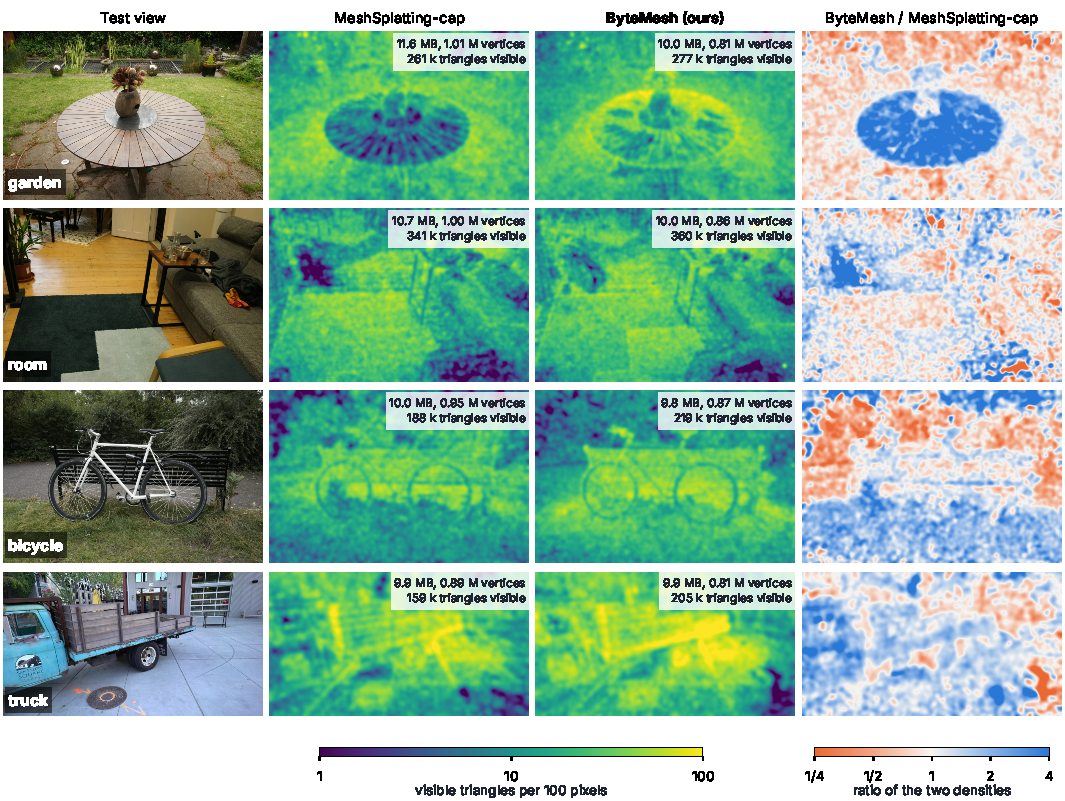
\includegraphics[width=\linewidth]{figures/fig_triangles_v5.pdf}
\caption{\textbf{Triangle density of \BM against \MSc at about the same file size}, on one test view of four scenes. Second and third column: visible triangles per 100 pixels; the corner gives the file size, the number of vertices and the number of triangles visible in the view. Last column: ratio of the two densities, blue where \BM has more triangles and orange where \MSc has more.}
\label{sup:fig:triangles}
\end{figure*}
Fig.~\ref{sup:fig:rd-all} shows the rate--distortion curves in PSNR, SSIM and LPIPS on each of the four datasets. At the same file size, \BM is better than \MSc with BM-Codec, and BM-Codec is better than the three baseline codecs, on every dataset and in every metric. Table~\ref{sup:tab:bd-metrics} gives the Bjontegaard deltas of \BM relative to \MSc in the three metrics. \BM is better on all 21 scenes in SSIM and in LPIPS.


\begin{table}[!htb]\centering\footnotesize
\caption{\textbf{Bjontegaard deltas of \BM relative to \MSc in three metrics}, both with BM-Codec; mean difference at the same file size, computed per scene and averaged. For LPIPS, lower is better.}
\label{sup:tab:bd-metrics}
\begin{tabular}{@{}lccc@{}}
\toprule
dataset (scenes) & PSNR (dB) & SSIM & LPIPS \\
\midrule
Mip-NeRF 360, T\&T (11) & $+0.30$ & $+0.012$ & $-0.017$ \\
Deep Blending (2) & $+0.23$ & $+0.007$ & $-0.008$ \\
NeRF-Synthetic (8) & $+0.29$ & $+0.003$ & $-0.004$ \\
all (21) & $+0.29$ & $+0.008$ & $-0.011$ \\
\bottomrule
\end{tabular}
\end{table}

\subsection{Where the triangles are}
Fig.~\ref{sup:fig:triangles} compares the triangles of \BM and of \MSc at about the same file size: 10~MB for \BM, and 10.0 to 11.6~MB for \MSc with the middle cap. For every pixel of a test view, we read from the renderer which triangle covers it. The local density is the number of visible triangles per pixel, averaged over a small neighborhood. The last column is the ratio of the two densities: blue where \BM has more triangles than \MSc, orange where it has fewer.

On the four views, \BM has 8\% to 20\% fewer vertices than \MSc and 6\% to 29\% more triangles visible in the view. It has at least 1.4 times the density of \MSc on 23\% to 42\% of the pixels, and at most 0.7 times on 8\% to 23\%. \BM moves triangles to the regions where the error is high. In the regions where \BM is denser, the mean $L_1$ error of \MSc is 0.044, 0.026, 0.066 and 0.048 (garden, room, bicycle, truck); in the regions where \BM is coarser, it is 0.039, 0.020, 0.030 and 0.038. On all four views, the error of \BM is below that of \MSc where \BM is denser, and above it where \BM is coarser. On garden, the difference is the table: \MSc covers it with large triangles.


\subsection{Codecs on the meshes from collapse after training}
Table~\ref{sup:tab:collapse-bd} extends Sec.~4.2 of the paper to \DeepBlending and \NeRFSyn. The order of the codecs is the same on the three groups of scenes. On \NeRFSyn each object has two or three vertex counts.

\begin{table}[!htb]\centering\footnotesize
\caption{\textbf{BD-rate of each codec relative to the meshes from collapse after training without a codec}, computed per scene and averaged.}
\label{sup:tab:collapse-bd}
\begin{tabular}{@{}lccc@{}}
\toprule
 & Mip-360, & Deep & NeRF- \\
codec & T\&T (11) & Blend.\ (2) & Synth.\ (8) \\
\midrule
Draco & $-56.0\%$ & $-28.4\%$ & $-7.4\%$ \\
zstd & $-81.8\%$ & $-76.7\%$ & $-79.5\%$ \\
MPEG TFAN & $-87.5\%$ & $-84.2\%$ & $-83.9\%$ \\
BM-Codec & $-95.1\%$ & $-94.2\%$ & $-90.0\%$ \\
\bottomrule
\end{tabular}
\end{table}

\subsection{File size against the vertex cap}
Fig.~\ref{sup:fig:cap} shows the file size of \MSc with BM-Codec for every scene and every cap. Over the 13 captured scenes, the files range from 5.8 to 7.5~MB at a cap of 0.6 million vertices, from 8.3 to 11.6~MB at 1.08 million, from 19.9 to 31.6~MB at 3 million and from 20.0 to 39.8~MB at the default cap of 4 million.

\begin{figure}[!htb]\centering
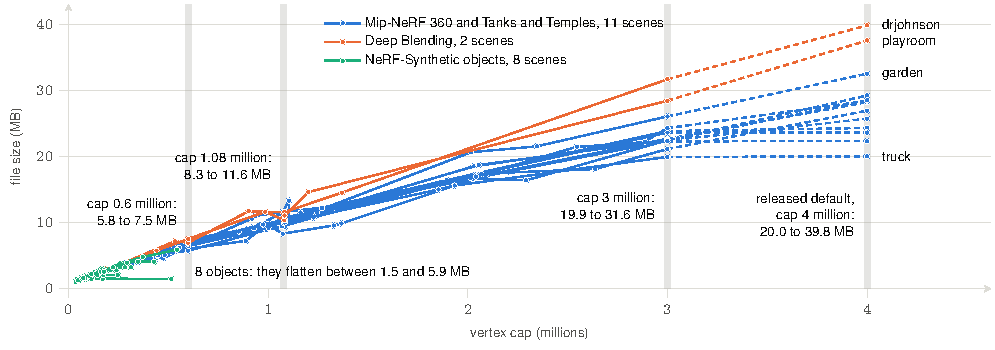
\includegraphics[width=\linewidth]{figures/fig_cap_instability.pdf}
\caption{\textbf{File size against the vertex cap}, one line per scene, BM-Codec. Dashed segments lead to the default cap of 4 million. The numbers on top give the range of file sizes over the 13 captured scenes at four caps.}
\label{sup:fig:cap}
\end{figure}

\subsection{Run-to-run variation}
Table~\ref{sup:tab:seeds} gives three runs with different random seeds on five scenes. The seed affects the training of \MS; the controller has no random component.

\begin{table}[!htb]\centering\footnotesize
\caption{\textbf{Run-to-run variation of \BM}: three runs with different random seeds, target 10~MB. The first run of each scene is the one reported in the paper.}
\label{sup:tab:seeds}
\setlength{\tabcolsep}{3pt}
\begin{tabular}{@{}lccc@{}}
\toprule
scene & file size (MB) & PSNR (dB) & range \\
\midrule
garden & 9.997 / 9.966 / 9.962 & 23.67 / 23.69 / 23.70 & 0.03 \\
bicycle & 9.784 / 9.811 / 9.809 & 22.51 / 22.53 / 22.50 & 0.03 \\
truck & 9.904 / 9.956 / 9.961 & 22.25 / 22.22 / 22.24 & 0.03 \\
kitchen & 10.014 / 10.029 / 10.023 & 26.41 / 26.31 / 26.45 & 0.15 \\
room & 9.992 / 9.896 / 9.958 & 27.99 / 27.76 / 27.92 & 0.23 \\
\midrule
mean & & 24.57 / 24.50 / 24.56 & 0.07 \\
\bottomrule
\end{tabular}
\end{table}

\subsection{\DeepBlending against Gaussian codecs}
Table~\ref{sup:tab:db-gs} places \BM next to published results of Gaussian codecs on \DeepBlending. As on \MipNeRF (Sec.~4.4 of the paper), the Gaussian codecs are better at the same file size; the gap is already present between \MS and 3DGS before compression.

\begin{table}[!htb]\centering\footnotesize
\caption{\textbf{\DeepBlending} (drjohnson, playroom); size in MB. Gaussian rows are published numbers collected in~\cite{hacpp2025}.}
\label{sup:tab:db-gs}
\setlength{\tabcolsep}{3.5pt}
\begin{tabular}{@{}lcccc@{}}
\toprule
method & PSNR & SSIM & LPIPS & MB \\
\midrule
3DGS~\cite{kerbl2023gaussians} & 29.42 & 0.899 & 0.247 & 663.9 \\
Compact3DGS~\cite{compact3dgs2024} & 29.79 & 0.901 & 0.258 & 43.2 \\
HAC++~\cite{hacpp2025}, low & 30.16 & 0.907 & 0.266 & 2.9 \\
HAC++, high & 30.34 & 0.911 & 0.254 & 5.3 \\
\midrule
\MS FP32~\cite{meshsplatting2025} & 27.23 & 0.842 & 0.337 & 772 \\
\midrule
\BM, 20 MB & 27.01 & 0.840 & 0.450 & 19.9 \\
\BM, 10 MB & 26.69 & 0.833 & 0.474 & 9.9 \\
\BM, 5 MB & 26.04 & 0.821 & 0.498 & 5.0 \\
\bottomrule
\end{tabular}
\end{table}

%=====================================================================
\section{Analysis of the codec}
\label{sup:codec}

\subsection{Where the bytes go}
Fig.~\ref{sup:fig:streams} shows the streams of the files of \BM at every target. On the 13 captured scenes at 10~MB, the connectivity takes 40\% of the file, the positions 22\%, the two SH indices 18\%, the DC color 13\% and the two codebooks 7\%. The shares change little with the target, except for the codebooks: they take 0.65~MB in every file, which is 13\% of a 5~MB file and 3\% of a 20~MB file. On \NeRFSyn the files are small, and the codebooks take 44\% of a 1.5~MB file.

Per vertex, a 10~MB file of a captured scene spends 39 bits on the connectivity (14.7 bits per face), 22 bits on the position, 17.6 bits on the two SH indices and 12.5 bits on the DC color. The 45 SH coefficients, which take 1{,}440 bits per vertex in 32-bit floats, are thus coded by 17.6 bits and a share of the codebooks.

\begin{figure}[!htb]\centering
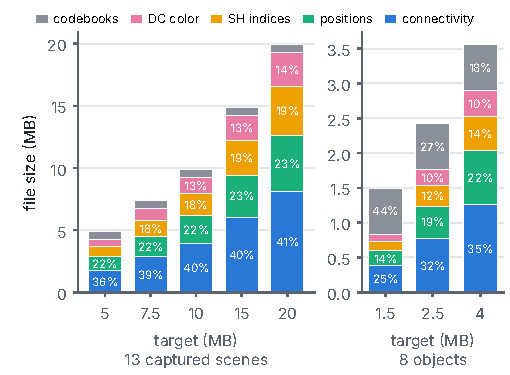
\includegraphics[width=\linewidth]{figures/fig_streams_v1.pdf}
\caption{\textbf{Composition of the files of \BM}: mean size of each stream over the scenes, at every target. The percentages are shares of the file.}
\label{sup:fig:streams}
\end{figure}

\subsection{Lossless coding against existing coders}
We keep the quantized mesh of BM-Codec and replace only the lossless coding (Table~\ref{sup:tab:lossless}). The decoded mesh is the same in every column, so the PSNR is the same. For MPEG TFAN and Draco, the DC color and the two indices are given as integer attributes, and the two codebooks are added as in BM-Codec. For zstd, each array is compressed at level 19, in the layout that gives the smallest result.

With the same quantized mesh, BM-Codec is smaller than MPEG TFAN on every one of the 21 scenes: by 11\% on average on the 13 captured scenes and by 8\% on \NeRFSyn. The larger gain over TFAN in Table~1 of the paper therefore comes from the vector quantization of the SH coefficients. zstd on the arrays in the order of the trained mesh gives files 78\% and 41\% larger; most of this difference comes from the order of the faces and vertices. Draco splits the vertices whose attributes differ between faces and decodes about five times as many vertices, so its files are about 2.8 times larger.

\begin{table}[!htb]\centering\footnotesize
\caption{\textbf{Same quantized mesh, different lossless coding.} Mean file size in MB; in brackets, the mean of the per-scene increase over BM-Codec.}
\label{sup:tab:lossless}
\begin{tabular}{@{}lcc@{}}
\toprule
lossless coding & captured (13) & NeRF-Synth.\ (8) \\
\midrule
BM-Codec & 10.36 & 2.37 \\
MPEG TFAN & 11.61 ($+12\%$) & 2.58 ($+9\%$) \\
zstd, order of BM-Codec & 12.29 ($+19\%$) & 2.63 ($+11\%$) \\
zstd, order of the trained mesh & 18.49 ($+78\%$) & 3.37 ($+41\%$) \\
Draco & 29.39 ($+183\%$) & 6.88 ($+184\%$) \\
\midrule
\multicolumn{3}{@{}l}{per stream, captured scenes (BM-Codec / zstd / zstd, trained order):} \\
connectivity & \multicolumn{2}{c}{3.64 / 4.95 / 9.73} \\
positions & \multicolumn{2}{c}{2.57 / 3.22 / 4.27} \\
SH indices & \multicolumn{2}{c}{2.02 / 2.11 / 2.28} \\
\bottomrule
\end{tabular}
\end{table}

\subsection{Design choices per dataset}
Table~\ref{sup:tab:choices} gives Table~7 of the paper for each group of scenes. Prediction from the mean of the earlier neighbors is the best choice for positions and for the DC color on every scene. For the SH indices, the neighbor candidates make the stream smaller on \DeepBlending (2 of 2 scenes) and \NeRFSyn (8 of 8), and larger on 7 of the 11 scenes of \MipNeRF and \TandT.

\begin{table}[!htb]\centering\footnotesize
\caption{\textbf{Codec design choices per dataset}, bits per vertex. The first row of each block is the codec used for all results.}
\label{sup:tab:choices}
\setlength{\tabcolsep}{3pt}
\begin{tabular}{@{}llccc@{}}
\toprule
 & & Mip-360, & Deep & NeRF- \\
attribute & coding method & T\&T (11) & Blend.\ (2) & Synth.\ (8) \\
\midrule
\multirow{4}{*}{positions} & one earlier neighbor & 22.6 & 25.4 & 30.6 \\
 & previous vertex & 23.2 & 26.0 & 30.8 \\
 & parallelogram & 23.5 & 26.5 & 31.9 \\
 & mean of earlier neighbors & 21.6 & 24.3 & 29.5 \\
\midrule
\multirow{2}{*}{DC color} & zstd, no prediction & 12.6 & 12.3 & 15.3 \\
 & mean of earlier neighbors & 11.3 & 10.0 & 13.1 \\
\midrule
\multirow{3}{*}{SH indices} & neighbors as candidates & 17.6 & 17.5 & 18.9 \\
 & no neighbor information & 17.4 & 17.9 & 19.3 \\
 & fixed length & 20.0 & 20.0 & 20.0 \\
\bottomrule
\end{tabular}
\end{table}

\subsection{Codebook size and DC precision}
Table~\ref{sup:tab:kr} and Fig.~\ref{sup:fig:kr} compare five sizes of the two codebooks on the 11 scenes of \MipNeRF and \TandT, at four file sizes. Without the residual codebook, the files are about 8\% smaller and the PSNR is 0.12 to 0.15\dB lower; at the same file size, this is 0.05 to 0.13\dB below the two codebooks. Codebooks of 16{,}384 and 1{,}024 codewords make the files 12\% to 49\% larger for a gain of 0.06 to 0.07\dB. The setting of the paper is at most 0.07\dB below the convex hull of all settings. With 8 bits for the DC color, the files are 4\% larger and the PSNR is 0.03\dB higher. The sweep was run on meshes from an earlier version of our training; the codec is the same.

\begin{table*}[!t]\centering\footnotesize
\caption{\textbf{Codebook size.} Change in file size and in PSNR (dB) against $K{=}4{,}096$, $L{=}256$, mean over 11 scenes, at four file sizes (size of the default file in the header).}
\label{sup:tab:kr}
\begin{tabular}{@{}lcccc@{}}
\toprule
$K + L$ & 4.5 MB & 9.4 MB & 20.4 MB & 27.0 MB \\
\midrule
4{,}096 + 0 & $-8.0\%$, $-0.12$ & $-8.4\%$, $-0.14$ & $-8.7\%$, $-0.15$ & $-8.9\%$, $-0.15$ \\
1{,}024 + 256 & $-12.8\%$, $-0.05$ & $-7.6\%$, $-0.05$ & $-5.0\%$, $-0.07$ & $-4.4\%$, $-0.07$ \\
4{,}096 + 256 & \multicolumn{4}{c}{reference} \\
4{,}096 + 1{,}024 & $+4.4\%$, $+0.02$ & $+3.3\%$, $+0.02$ & $+2.7\%$, $+0.03$ & $+2.7\%$, $+0.03$ \\
16{,}384 + 1{,}024 & $+49\%$, $+0.06$ & $+27\%$, $+0.06$ & $+15\%$, $+0.07$ & $+12\%$, $+0.07$ \\
\bottomrule
\end{tabular}
\end{table*}

\begin{figure}[!htb]\centering
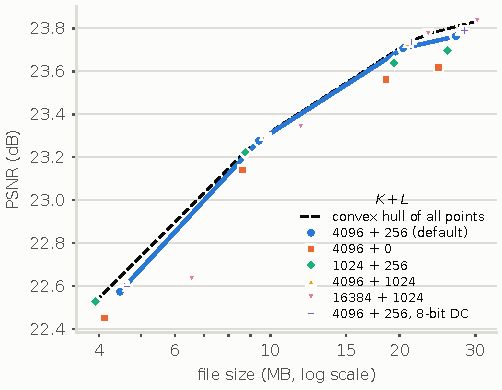
\includegraphics[width=\linewidth]{figures/fig_codebook_sweep_v2.pdf}
\caption{\textbf{Codebook size.} Each point is the mean over 11 scenes of one mesh size (four sizes) and one codec setting (six settings). Dashed: convex hull of all 24 points. Blue line: the setting of the paper.}
\label{sup:fig:kr}
\end{figure}

\subsection{Coding time and refinement per dataset}
Table~\ref{sup:tab:time} extends Table~4 of the paper. All codecs are timed on the same CPU node; the vector quantization runs on a GPU. On \NeRFSyn a mesh has about 0.13 million vertices, and the encoding takes 19~s.

\begin{table}[!htb]\centering\footnotesize
\caption{\textbf{Coding time of BM-Codec per dataset} (seconds, mean over the scenes), and gain of the codeword refinement in PSNR on the test views. \MSc meshes with the middle cap.}
\label{sup:tab:time}
\setlength{\tabcolsep}{3pt}
\begin{tabular}{@{}lccc@{}}
\toprule
 & Mip-360, & Deep & NeRF- \\
 & T\&T (11) & Blend.\ (2) & Synth.\ (8) \\
\midrule
$k$-means & 2.6 & 2.5 & 1.0 \\
assignment & 5.7 & 5.5 & 6.9 \\
refinement (400 steps) & 47.7 & 38.0 & 10.6 \\
entropy coding & 4.6 & 5.3 & 0.9 \\
\midrule
encoding, total & 60.7 & 51.3 & 19.4 \\
decoding & 3.7 & 4.1 & 0.8 \\
\midrule
gain of the refinement (dB) & 0.25 & 0.32 & 0.16 \\
\bottomrule
\end{tabular}
\end{table}

%=====================================================================
\section{Analysis of the rate-controlled training}
\label{sup:training}

\subsection{Where the gain comes from}
We run \BM with Phase~2 turned off: the growth aims at the target ($\alpha = 1$) and no edge is collapsed. Table~\ref{sup:tab:p1} gives the result on five scenes at 5, 10 and 20~MB. Without Phase~2, the files end at 77\% to 96\% of the target. Against \MSc, this variant gives a BD-PSNR of $+0.19$\dB on average, and \BM gives $+0.35$\dB on the same five scenes. The split by error (Phase~1) and the growth past the target followed by collapses (Phase~2) therefore each contribute about half of the gain. Phase~2 is also what makes the file reach the target.

\begin{table}[!htb]\centering\footnotesize
\caption{\textbf{Phase~1 only.} File size divided by the target at 5 / 10 / 20~MB, and BD-PSNR (dB) relative to \MSc, for Phase~1 alone and for \BM. One run each; all meshes written by BM-Codec.}
\label{sup:tab:p1}
\setlength{\tabcolsep}{3.5pt}
\begin{tabular}{@{}lccc@{}}
\toprule
 & size / target, & \multicolumn{2}{c}{BD-PSNR vs.\ \MSc} \\
scene & Phase 1 only & Phase 1 only & \BM \\
\midrule
garden & 0.83 / 0.85 / 0.84 & $+0.09$ & $+0.22$ \\
room & 0.86 / 0.86 / 0.83 & $+0.16$ & $+0.38$ \\
bicycle & 0.78 / 0.79 / 0.78 & $+0.33$ & $+0.37$ \\
kitchen & 0.91 / 0.96 / 0.96 & $+0.34$ & $+0.68$ \\
truck & 0.81 / 0.81 / 0.77 & $+0.01$ & $+0.11$ \\
\midrule
mean & & $+0.19$ & $+0.35$ \\
\bottomrule
\end{tabular}
\end{table}

\subsection{Growth aim on every scene}
Table~\ref{sup:tab:alpha} gives the runs behind Table~6 of the paper.

\begin{table}[!htb]\centering\footnotesize
\caption{\textbf{Growth aim $\alpha$ on every scene}: file size (MB) / PSNR (dB), target 10~MB, one run each.}
\label{sup:tab:alpha}
\setlength{\tabcolsep}{3pt}
\begin{tabular}{@{}lcccc@{}}
\toprule
scene & $\alpha=1.0$ & $1.2$ & $1.35$ & $1.5$ \\
\midrule
garden & 8.46 / 23.33 & 9.94 / 23.57 & 10.00 / 23.67 & 9.96 / 23.76 \\
room & 8.72 / 27.65 & 10.03 / 27.90 & 9.99 / 27.99 & 9.70 / 27.84 \\
bicycle & 7.90 / 22.31 & 9.45 / 22.43 & 9.78 / 22.51 & 9.82 / 22.53 \\
kitchen & 9.51 / 26.14 & 10.05 / 26.36 & 10.01 / 26.41 & 10.02 / 26.37 \\
truck & 8.08 / 22.01 & 9.66 / 22.20 & 9.90 / 22.25 & 9.92 / 22.31 \\
\bottomrule
\end{tabular}
\end{table}

\subsection{Why the file reaches the target}
Let $R_k$ be the file size that the probe measures at round $k$ of Phase~2, and $c_k$ the bytes that the collapses of this round remove according to Eq.~(2) of the paper. Until the next round, the training changes the size by a drift $d_k$: the opacity rises, vertices move, and \MS prunes triangles. With $\epsilon_k$ the error of the linear model,
\begin{equation}
R_{k+1} = R_k - c_k + d_k + \epsilon_k .
\end{equation}
Each round removes the whole measured excess, $c_k = \max(R_k - T,\, 0)$. Whenever $R_k \ge T$, this gives
\begin{equation}
R_{k+1} - T = d_k + \epsilon_k .
\label{sup:eq:excess}
\end{equation}
Three properties follow. First, the excess at a round depends only on what happened since the previous round. Errors of earlier rounds do not accumulate, and no prediction of the future size is needed. Second, the final error is the drift after the last round, plus the difference between the probe and the final encoder. Third, the controller can only remove bytes. A mesh below the target reaches it only through the drift.

Fig.~\ref{sup:fig:traces} shows the measured size at every round for the 65 runs on the 13 captured scenes. 40 runs are above the target at the first round, by up to 23\%, and are brought to it in one or two rounds. The other 25 runs start below the target, by up to 20\%. Their size rises during training, because the opacity rises and more faces become visible; the collapses start once the target is reached. In the 1{,}083 cases where a round measures a size at or above the target, the size at the next round is within 1.9\% of the target in 95\% of the cases (median $+0.4\%$). On average, 17 of the 35 rounds collapse edges. In the last rounds the size decreases slightly, and nothing adds bytes: at 30k the measured size is between 94\% and 101\% of the target (99\% on average). When the growth of Phase~1 is too small, the size never reaches the target: this is the case with $\alpha = 1$ (Table~\ref{sup:tab:alpha}), and for ficus and mic, which stop growing.

The probe builds its codebooks without the refinement. On the 39 runs at 5, 10 and 20~MB, the probe at the end of training is within 0.32\% of the file that the final encoder writes.

\begin{figure}[!t]\centering
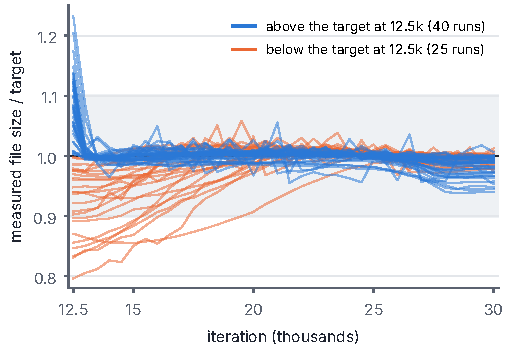
\includegraphics[width=\linewidth]{figures/fig_controller_traces_v2.pdf}
\caption{\textbf{Measured file size during Phase~2}, divided by the target, for the 65 runs on the 13 captured scenes (five targets). One line per run; the last point is the size at 30k. Grey band: $\pm10\%$.}
\label{sup:fig:traces}
\end{figure}

\subsection{Time of the full pipeline}
Table~\ref{sup:tab:pipeline} gives the time of each stage. One training run has 41 or 42 size probes. Over the 65 runs on the 13 captured scenes, the probes take at least 41\% of the training time on average (30\% to 50\%), about 20 minutes per run.

\begin{table}[!htb]\centering\footnotesize
\caption{\textbf{Time of each stage of \BM.} Training, conversion and fine-tuning: mean over the 13 captured scenes, one L40S GPU. Coding: mean over the 11 scenes of \MipNeRF and \TandT (Table~4 of the paper). Rendering: garden and bicycle, WebGL on a laptop (Sec.~4.4 of the paper).}
\label{sup:tab:pipeline}
\begin{tabular}{@{}lc@{}}
\toprule
stage & time \\
\midrule
rate-controlled training, 30k iterations & 48.8 min \\
\quad of which size probes & about 20 min \\
removal of hidden faces and conversion & 2.0 min \\
fine-tuning, 3{,}000 iterations & 3.2 min \\
encoding (codebooks and file) & 60.7 s \\
decoding & 3.7 s \\
rendering one frame, 5 / 10 / 20 MB & 1.0 / 1.3 / 2.0 ms \\
\bottomrule
\end{tabular}
\end{table}

%=====================================================================
\section{Qualitative comparison with error maps}
\label{sup:qual}

Fig.~\ref{sup:fig:qual} extends Fig.~2 of the paper to full test views of four scenes, with the error of each render. At about 10~MB, \MSc with TFAN loses the colors, because the SH coefficients are quantized coarsely. Collapse after training keeps the colors and loses geometry: the error is concentrated on edges and thin structures. The error map of \BM is the closest to that of the FP32 model.

\begin{figure*}[!tp]\centering
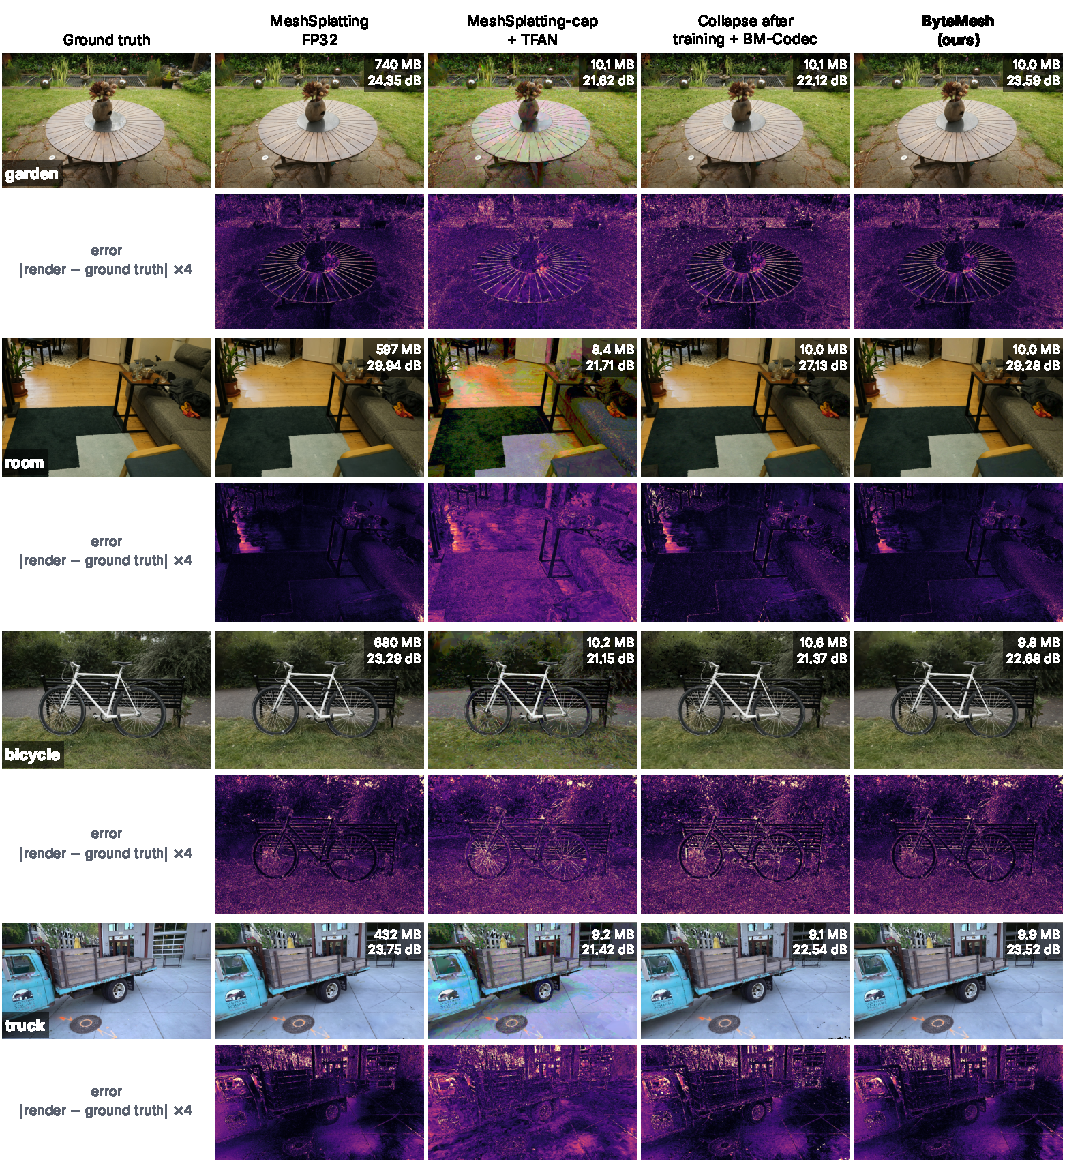
\includegraphics[width=\linewidth]{figures/fig_qual_error_v1.pdf}
\caption{\textbf{Full views and error maps at the same file size} (about 10~MB) on garden, room, bicycle and truck. First row of each scene: the test view. Second row: $|\text{render} - \text{ground truth}|$, mean over the color channels, multiplied by 4. The corner of each render gives the file size and the PSNR of this view.}
\label{sup:fig:qual}
\end{figure*}
